\section{Crucial elements of the \texttt{MIMUW-MB-TT} plugin}

\subsection{The internal system}\label{subsec:internal_system}

The main component of the internal system are the two buffers filled with the intervals. One of these buffers is the live buffer. The live buffer contains the data gathered lately. It is responsible for creating new intervals from the data that is coming from the user in the real time. The tool remembers to save the data in the file system in order to preserve it and not lose it all after potential crashes or closing the tool. After saving the data it is possible to remove some intervals from the live buffer in order to be aware of its size and not to allow it to get too big and clog the memory. The other of the buffers is the static buffer. It is responsible for loading the data from the file system in order for it to be then transferred to the dashboard. The user can request the data from the dashboard.

\begin{figure}[ht]
  \centering
  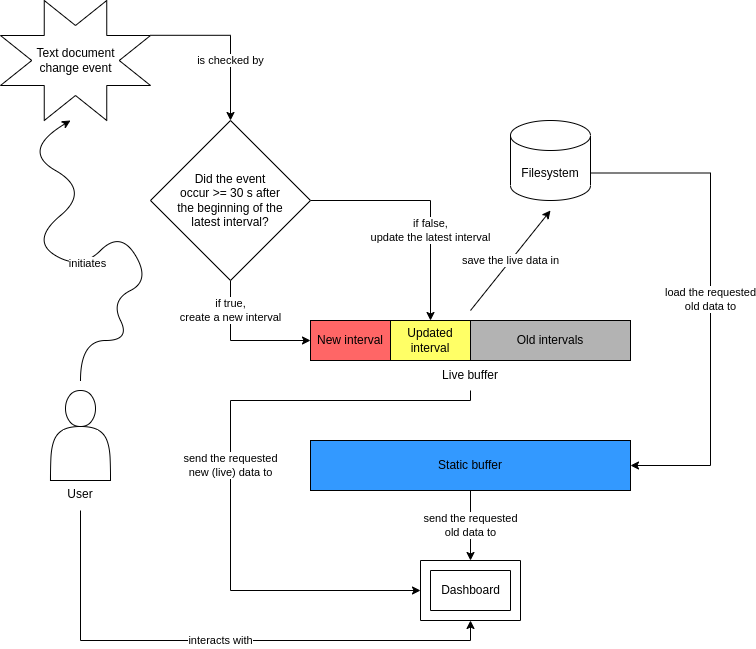
\includegraphics[scale=0.4]{chapters/methodology/graphics/internal-system.png}
  \caption{Internal system}
  \label{fig:internal_system}
\end{figure}

In order for for the intervals to be visualized they need to be normalized that is made to be of equal lengths. But the raw data consists of the intervals of varying lengths that is of length at most 30 seconds. I need to adjust them to be even-sized. Normalization recognizes also that the intervals need to stick to each other, however in the raw data there may exist breaks, since there are situations where for some time a user may be inactive. So essentially I can treat the time spaces that are not covered by the data as intervals with zero keystrokes. Then by interpreting this data such way I can proceed with interpolation (as shown in the example \ref{fig:internal_system}). Let me imagine that I split the requested time space into intervals of equal length and then I check if they intersect with the intervals from the real data. The amount of keystrokes that the new interval receives is proportional to the relative size of the intersection to the length of the whole row interval.
% So it's about you looking at the example from the figure if the intersection constitutes 30\% of the row interval then then we take into account 30\% of keystrokes from this row interval to the new interval of equivalent.
The total number of keystrokes associated with this new interval is calculated by summing all of the keystrokes associated with all the intersections from the different row intervals.

\begin{figure}[htbp]
  \centering
  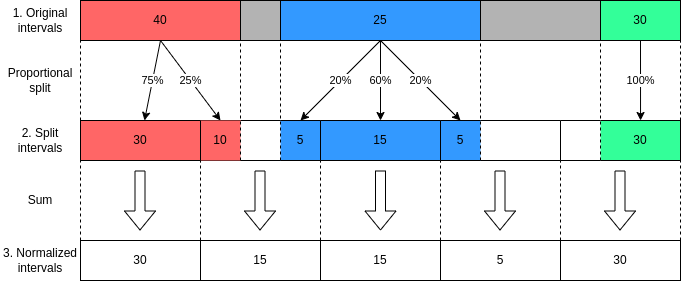
\includegraphics[scale=0.5]{chapters/methodology/graphics/normalization.png}
  \caption{An intervals normalization example}
  \label{fig:normalization_example}
\end{figure}

\subsection{Dashboard (UI)}

The dashboard constitutes the user interface that a user can use to view various statistics across different time periods. It is possible through switching modes. The first mode is called the live view \ref{fig:live_view}. In this view the user is able to view the latest data. Hovering over the data points on the plot (green or red dots on the line) reveals a tooltip containing more details (mainly the exact numerical values of the respected data point). The user can also adjust the time gauge to explore the data in the different time periods (last 10, 30 or 60 minutes from the current time). Moreover, he is provided with the Calendar view \ref{fig:calendar_view}. It is utilized to explore the data from previous days. After selecting the current day the user can also adjust the time period by using the aforementioned gauges. The parameters of the plot are adjusted automatically in order for the plot to be clearly visible to the user. This means to be not too convoluted and not too cluttered. The dashboard is connected with the live and static buffers and depending on the view the data is loaded from the live buffer or from the static buffer (that is indirectly from the file system). It is possible through the day view \ref{fig:day_view} that is accessible by selecting a day in the calendar view.

Users are enabled to save and upload the data manually by clicking on the buttons in the upper-right corner of either of the views. Since the quota of API calls to Dropbox servers is limited with my subscription plan, I have implemented a cooldown period on subsequent manual uploads to conserve the available API invocations.

\begin{figure}[htbp]
  \centering
  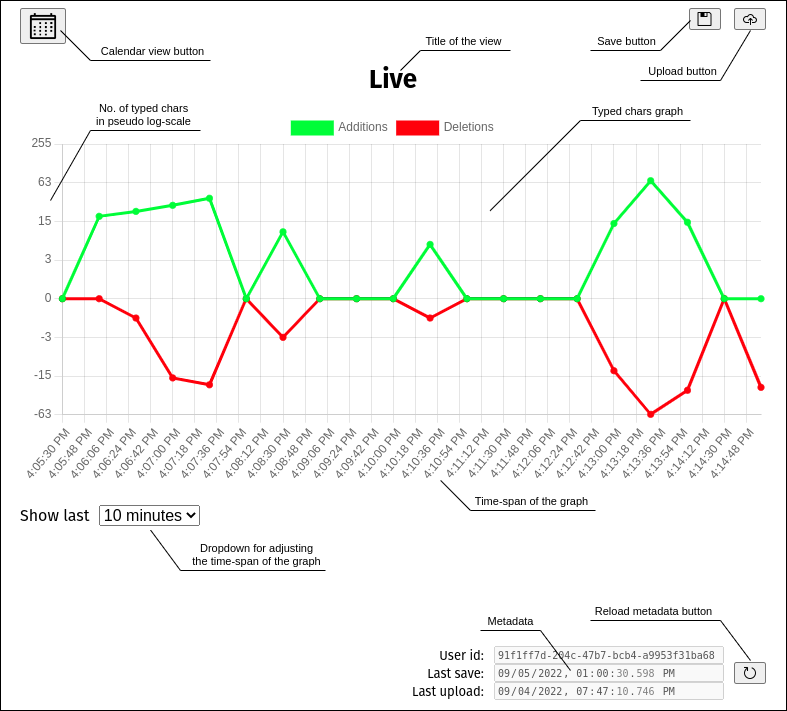
\includegraphics[scale=0.4]{chapters/methodology/graphics/live-view.png}
  \caption{Live view of the dashboard}
  \label{fig:live_view}
\end{figure}

\begin{figure}[htbp]
  \centering
  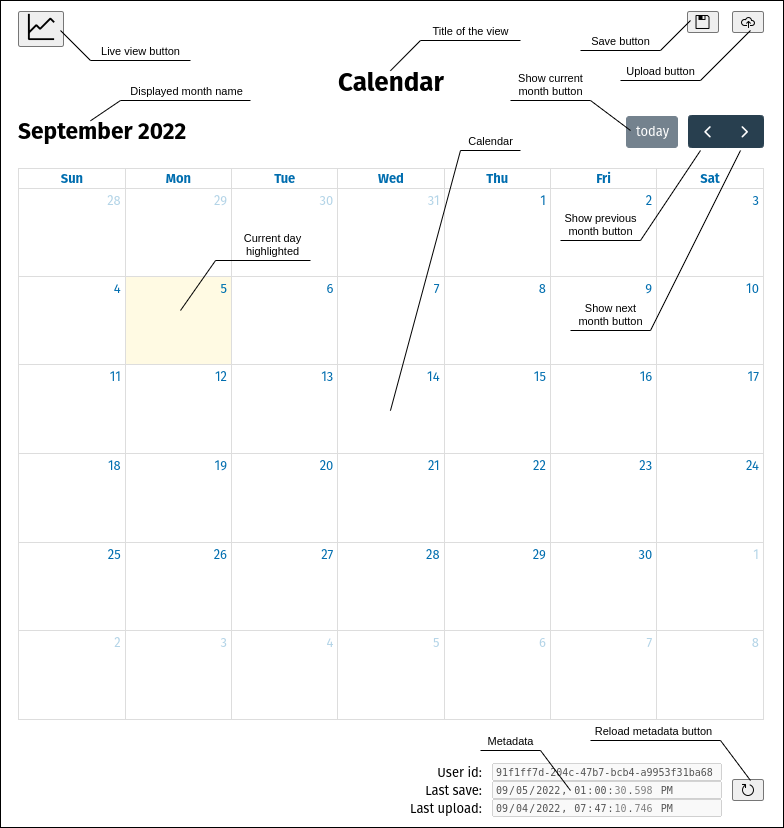
\includegraphics[scale=0.4]{chapters/methodology/graphics/calendar-view.png}
  \caption{Calendar view of the dashboard}
  \label{fig:calendar_view}
\end{figure}

\begin{figure}[htbp]
  \centering
  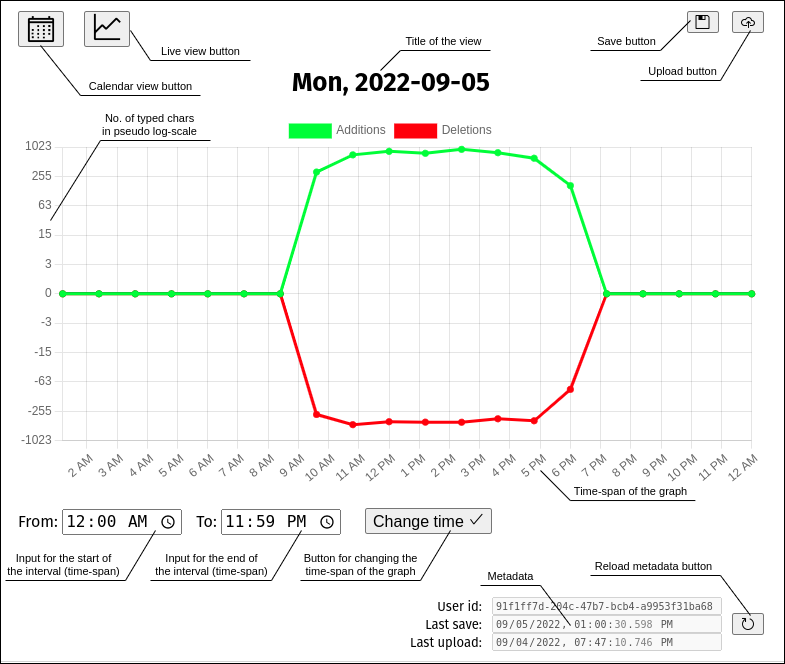
\includegraphics[scale=0.4]{chapters/methodology/graphics/day-view.png}
  \caption{Day view of the dashboard}
  \label{fig:day_view}
\end{figure}
